% ============================================== %

%%%%%%%%%%%%%%%%%%%%%%%%%%%%%%%%%%%%%%%%%%%%%%%%%%
%%%			  08 Trabalho Prático 08		   %%%
%%%%%%%%%%%%%%%%%%%%%%%%%%%%%%%%%%%%%%%%%%%%%%%%%%

% ============================================== %

\section{Trabalho Prático 08}

Para a treliça espacial simétrica de 3 barras, pede-se fazer gráficos $P\times\delta_v$ (
deslocamento vertical) e $P\times N$ (força axial nas barras) considerando-se $y \in [-4; 2]$
m usando as cinco leis constitutivas que relacionam linearmente as medidas de deformação
clássicas e seus respectivos pares conjugados de tensão. Adotar:

$$
\left\{\begin{array}{lcl}
	EA_0 &=& 133,865\text{ kN} \\
	H &=& 200\text{ cm} \\
	L &=& 500\text{ cm} \\
	\Delta y &=& -0,02\text{ m} \\
\end{array}\right.
$$

\begin{figure}[H]
	\centering
	\caption{Sistema estrutural do Trabalho Prático 08 -- Vista superior}
	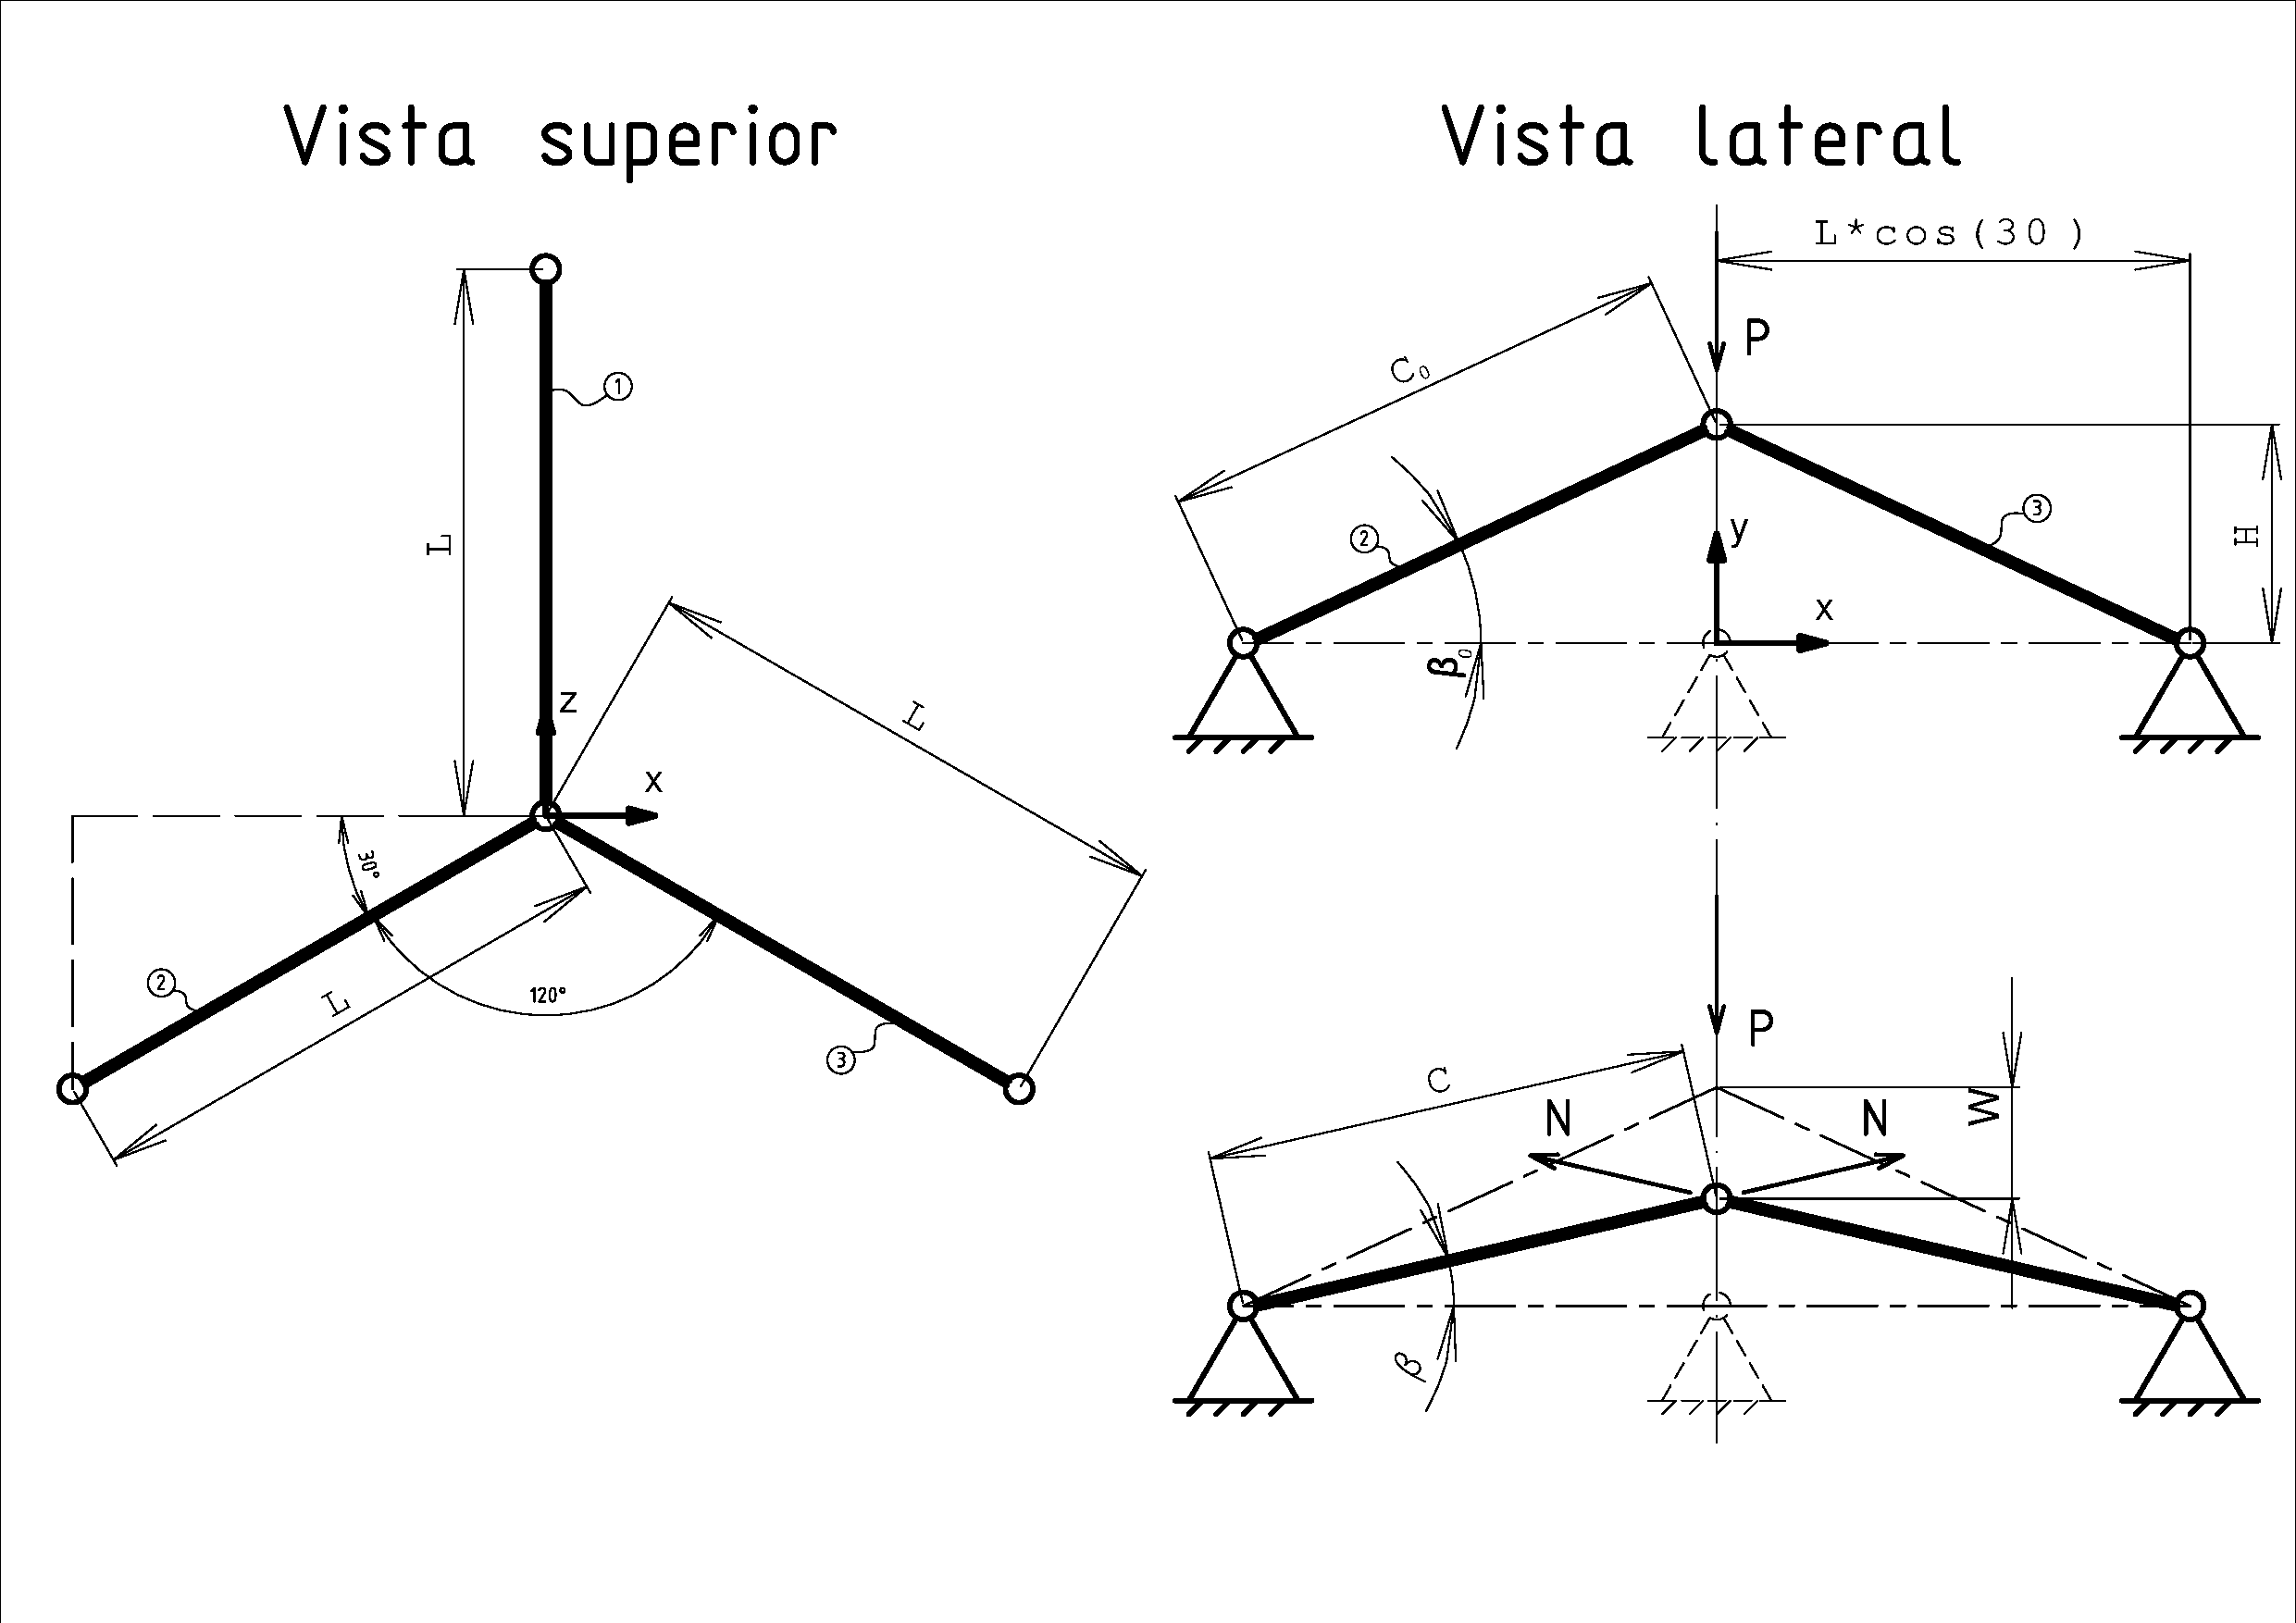
\includegraphics[
		trim=8mm 75mm 210mm 40mm,
		clip,
		width=0.75\textwidth
	]{figuras/TPs-8.pdf}
\end{figure}

\begin{figure}[H]
	\centering
	\caption{Sistema estrutural do Trabalho Prático 08 -- Vista lateral}
	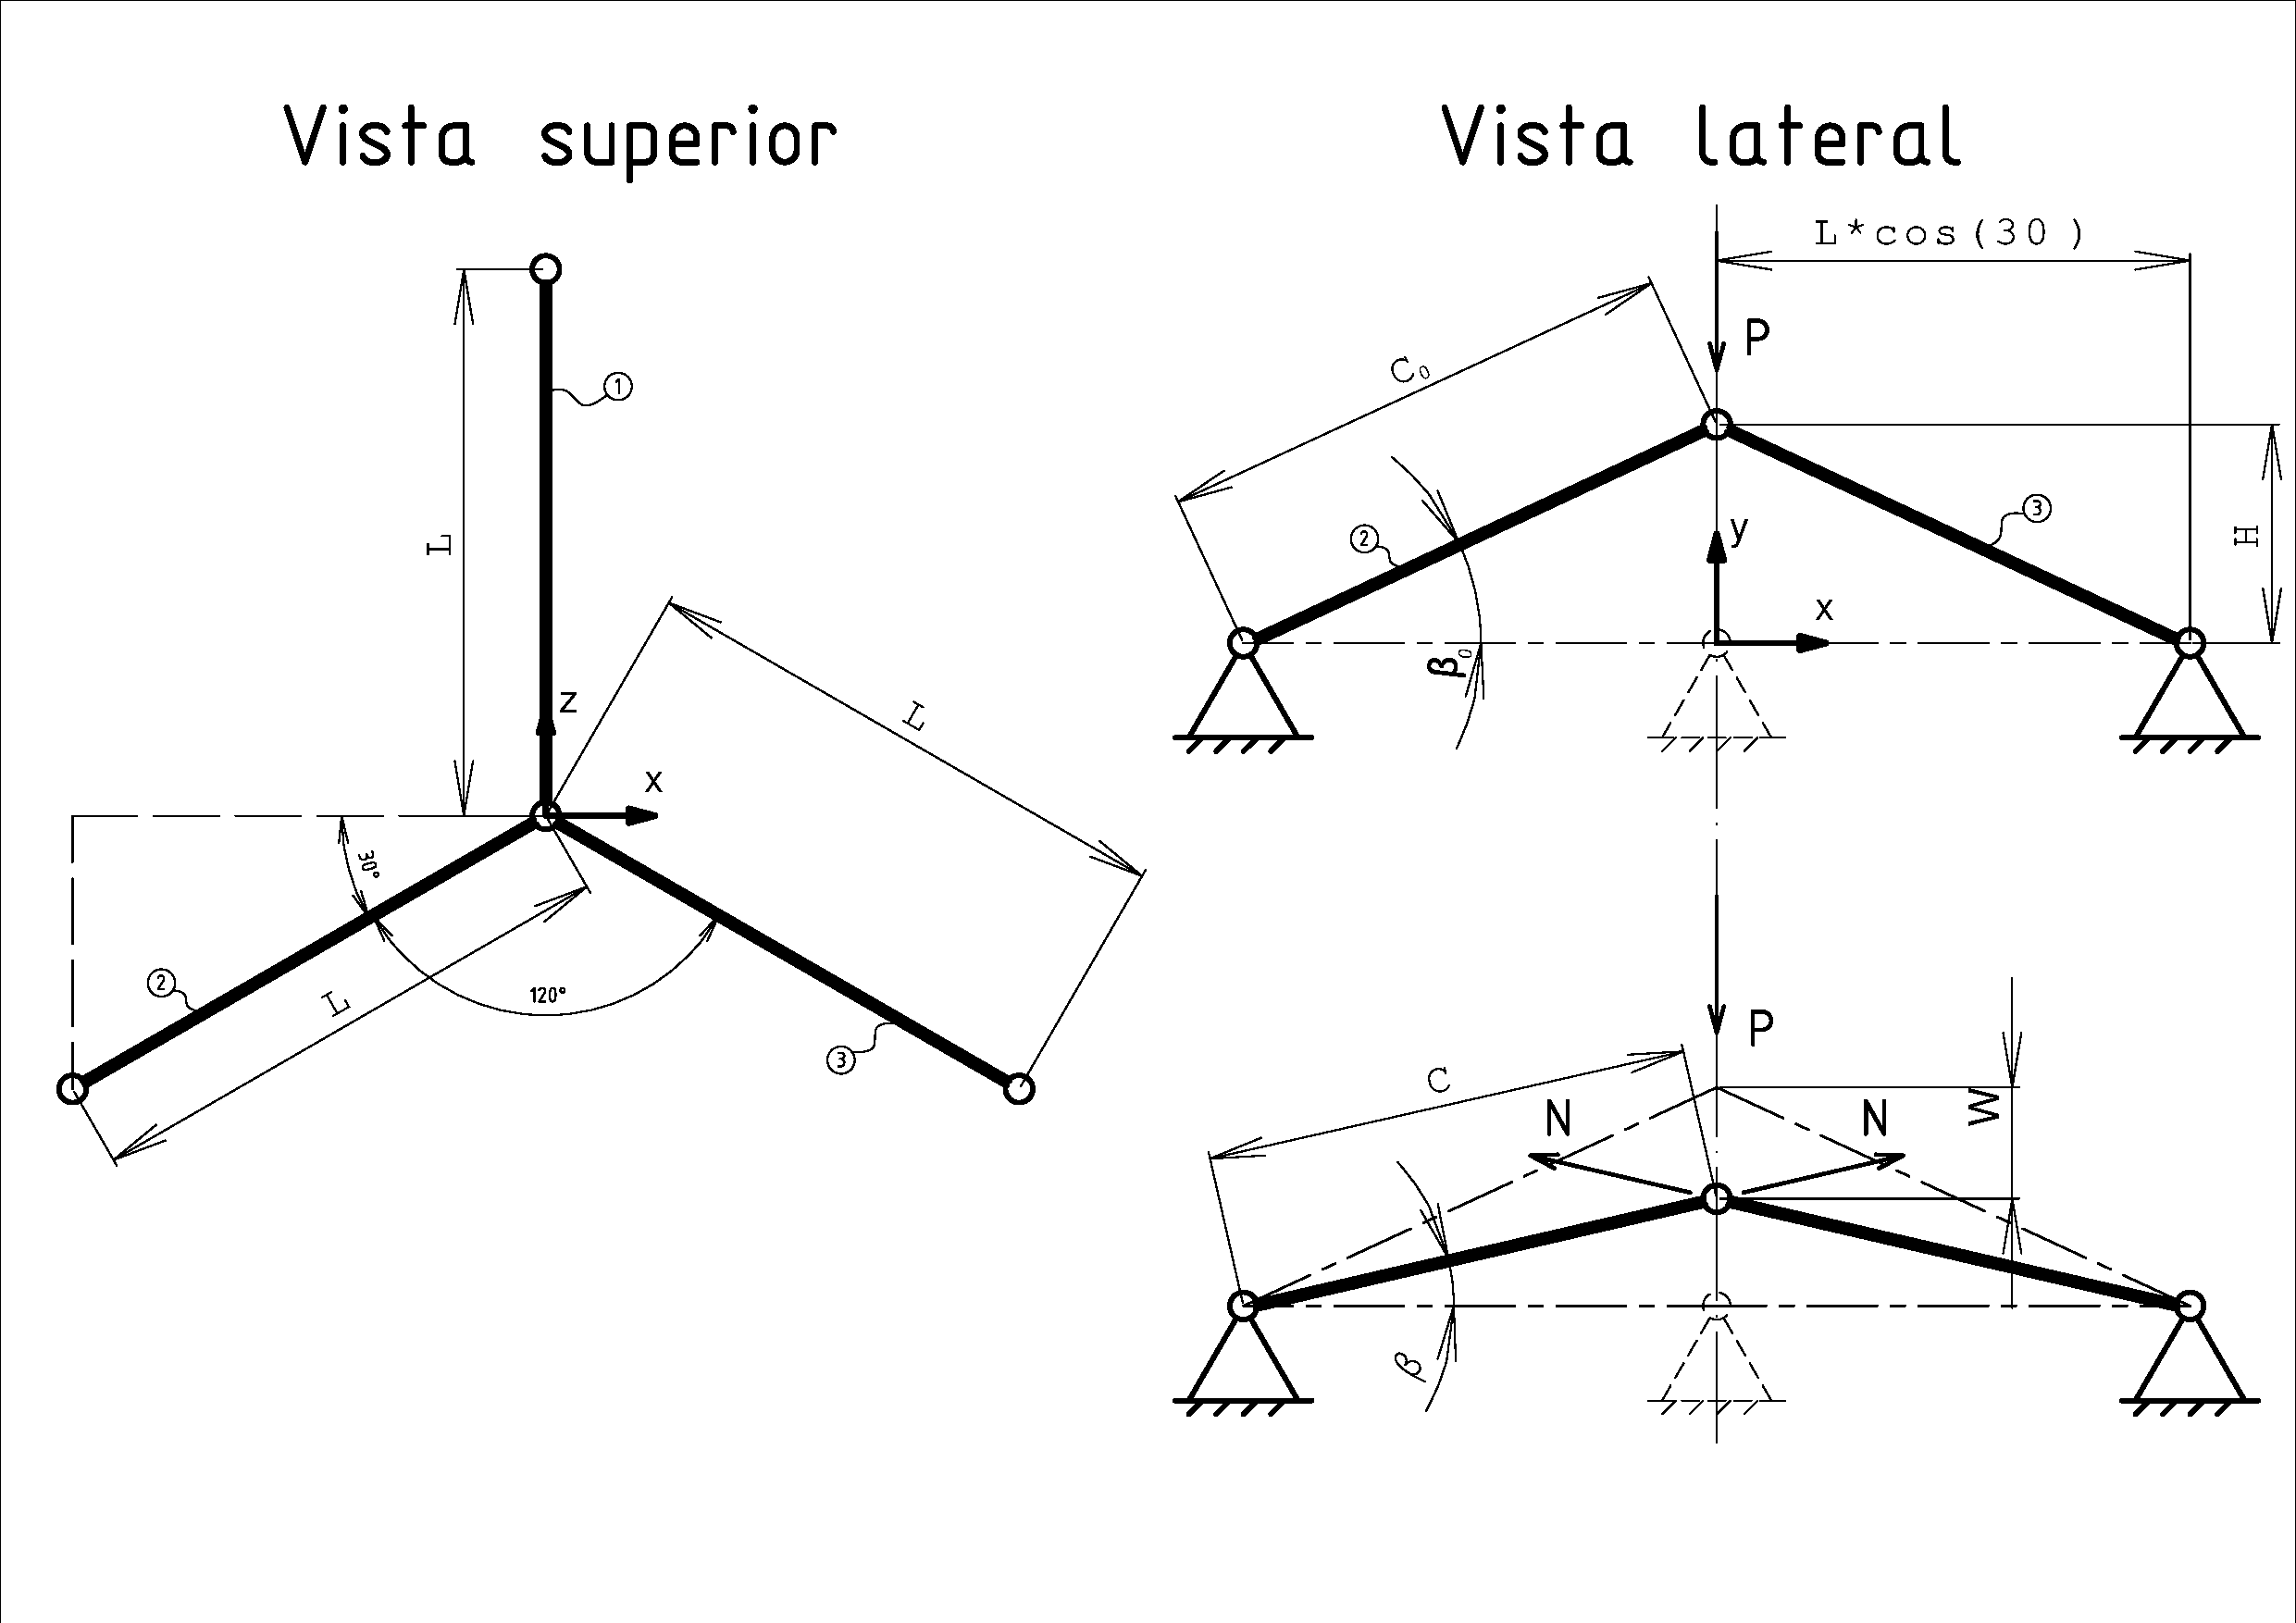
\includegraphics[
		trim=210mm 35mm 1.5mm 35mm,
		clip,
		width=0.85\textwidth
	]{figuras/TPs-8.pdf}
\end{figure}


% ================ Resolução TP-08 ================
\begin{textocaixa}
\hspace{10mm}

A treliça espacial do problema possui simetria radial, de modo que a força normal
$\vv{N} = \left(N_x\,\hat{i} + N_y\,\hat{j} + N_z\,\hat{k}\right)$, atuante na direção axial
de cada barra, possui o mesmo módulo para todas as barras. No \underline{equilíbrio}, a
resultante nas direções $x$ e $z$ das forças normais se cancelam, de modo que a equação de
equilíbrio se torna:

\begin{equation}
	3N_y - P = 0
	\label{eq:TP8-equi_init}
\end{equation}

Denotando por $\vv{v_1}$ o vetor direção da barra $\circled{1}$ na configuração deformada,
$\alpha$ o ângulo entre o vetor normal $\vv{N}$ e a vertical, e $N = ||\vv{N}||$,
tem-se que:

\begin{equation}
	\boxed{N_y = N\cos\alpha}
	\label{eq:TP8-Ny}
\end{equation}

\begin{equation}
	\cos\alpha = \frac{\left<\vv{v_1}, y\,\hat{j}\right>}
					  {||\vv{v_1}||\cdot
					   ||y\,\hat{j}||}
	= \frac{\left(0, y, L\right)\cdot\left(0, y, 0\right)}
		   {\sqrt{y^2 + L^2}\cdot y}
	\longrightarrow \boxed{\cos\alpha = \frac{y}{\sqrt{y^2 + L^2}}}
	\label{eq:TP8-cos_alpha}
\end{equation}

Por simetria, o ângulo $\alpha$ será igual para todas as barras. Assim, a equação final do
equilíbrio é dada por

\begin{equation}
	\boxed{N = -\frac{P}{3\cos\alpha}}
	\label{eq:TP8-equi}
\end{equation}

Além disso, as medidas de deformação clássicas (família Seth-Hill) se baseiam no estiramento
$\lambda$ da barra, no caso 1D, o qual é calculado como a razão entre o comprimento $c$ da
barra na configuração deformada e o comprimento $c_0$ da barra na configuração inicial:

\begin{equation}
	\lambda = \frac{c}{c_0}
	\label{eq:TP8-estiramento_init}
\end{equation}

Dimensões essas que se relacionam com os ângulos $\beta$ e $\beta_0$ baseando-se na
\underline{compatibilidade cinemática} do problema, dada na \autoref{eq:TP8-cinem}.

\begin{bigEquation}
	\left\{\begin{array}{lclcl}
		\tan\beta_0 &=& \frac{H}{L}    & & \\ [10pt]
		\tan\beta   &=& \frac{y}{L}    & & \\ [10pt]
		c_0			&=& L\,\sec\beta_0 &=& \sqrt{L^2 - H^2} \\ [10pt]
		c			&=& L\,\sec\beta   &=& \sqrt{L^2 - y^2}\\ [10pt]
	\end{array}\right.
	\label{eq:TP8-cinem}
\end{bigEquation}

Dessa forma, o estiramento se relaciona com os ângulos $\beta$ e $\beta_0$ de forma
não-linear, como mostrado na \autoref{eq:TP8-estiramento}.

\begin{equation}
	\lambda = \frac{c}{c_0} = \frac{L\,\sec\beta}{L\,\sec\beta_0}
	\longrightarrow \boxed{\lambda = \frac{\cos\beta_0}{\cos\beta}}
	\label{eq:TP8-estiramento}
\end{equation}

Ou, em termos das dimensões $L$, $H$ e $y$:

\begin{equation}
	\boxed{\lambda = \sqrt{\frac{\displaystyle 1 - \left(\frac{y}{L}\right)^2}
								{\displaystyle 1 - \left(\frac{H}{L}\right)^2}}}
	\label{eq:TP8-estiramento_alt}
\end{equation}

Enquanto o conjugado de tensão de cada medida de deformação se relaciona com a tensão de
Biot $\sigma_B$, a qual vale:

\begin{equation}
	\boxed{\sigma_B = \frac{N}{A_0}}
	\label{eq:TP8-sigmaB}
\end{equation}

Abaixo, serão construídas relações entre a carga $P$ e a coordenada $y$ do nó 4 (nó central)
para cada uma das cinco \underline{relações constitutivas} da família de Seth-Hill.

\begin{itemize}
	\item[a)] \underline{Green ($m = 2$)}
	
	$$\sigma_G = \frac{1}{\lambda}\cdot\sigma_B = E\cdot\varepsilon_G$$
	$$\frac{1}{\lambda}\cdot\frac{N}{A_0} = E\cdot\frac{1}{2}\left(\lambda^2 - 1\right)$$
	$$-\frac{P}{\lambda\cdot 3A_0\cos\alpha} = \frac{E}{2}\left(\lambda^2 - 1\right)$$
	
	\begin{equation}
		\boxed{P = -\frac{3EA_0\,\cos\alpha}{2}\cdot\lambda\left(\lambda^2 - 1\right)}
		\label{eq:TP8-P_Green}
	\end{equation}

	\item[b)] \underline{Biot ($m = 1$)}:
	
	$$\sigma_B = E\cdot\varepsilon_B$$
	$$\frac{N}{A_0} = E\cdot \left(\lambda - 1\right)$$
	$$-\frac{P}{3A_0\cos\alpha} = E\left(\lambda - 1\right)$$

	\begin{equation}
		\boxed{P = -\,3EA_0\,\cos\alpha\,\left(\lambda - 1\right)}
		\label{eq:TP8-P_Biot}
	\end{equation}
	
	\item[c)] \underline{Logarítmica ($m = 0$)}
	
	$$\sigma_L = \lambda\cdot\sigma_B = E\cdot\varepsilon_L$$
	$$\lambda\cdot\frac{N}{A_0} = E\cdot\ln\lambda$$
	$$-\frac{\lambda\cdot P}{3A_0\cos\alpha} = E\cdot\ln\lambda$$

	\begin{equation}
		\boxed{P = -\,3EA_0\,\cos\alpha\cdot\frac{\ln\lambda}{\lambda}}
		\label{eq:TP8-P_Logaritmica}
	\end{equation}
	
	\item[d)] \underline{Hiperbólica ($m = -1$)}
	
	$$\sigma_H = \lambda^2\cdot\sigma_B = E\cdot\varepsilon_H$$
	$$\lambda^2\cdot\frac{N}{A_0} = E\cdot\left(1 - \frac{1}{\lambda}\right)$$
	$$-\frac{\lambda^2\cdot P}{3A_0\cos\alpha} = E\cdot\left(1 - \frac{1}{\lambda}\right)$$

	\begin{equation}
		\boxed{P = -\,3EA_0\,\cos\alpha\cdot\frac{\lambda - 1}{\lambda^3}}
		\label{eq:TP8-P_Hiperbolica}
	\end{equation}
	
	\item[e)] \underline{Almansi ($m = -2$)}
	
	$$\sigma_A = \lambda^3\cdot\sigma_B = E\cdot\varepsilon_A$$
	$$\lambda^3\cdot\frac{N}{A_0} = E\cdot\left(1 - \frac{1}{\lambda^2}\right)$$
	$$-\frac{\lambda^3\cdot P}{3A_0\cos\alpha} = E\cdot\left(1 - \frac{1}{\lambda^2}\right)$$

	\begin{equation}
		\boxed{P = -\,3EA_0\,\cos\alpha\cdot\frac{\lambda^2 - 1}{\lambda^5}}
		\label{eq:TP8-P_Almansi}
	\end{equation}

\end{itemize}

Para a implementação numérica, seguiu-se o passo a passo abaixo:

\begin{enumerate}
	\item Calcular $\cos\beta_0$;
	\item Dado um $y_i = y_{i-1} + \Delta y$, calcular e armazenar:
	\begin{enumerate}[
		align=left
	]
		\item[(i)] deslocamento vertical $\delta_v = H - y$;
		\item[(ii)] $\cos\alpha$;
		\item[(iii)] constante $k \overset{\Delta}{=} 3EA_0\,\cos\alpha$;
		\item[(iv)] $\cos\beta$;
		\item[(v)] estiramento $\lambda$;
		\item[(vi)] carga $P$ que equilibra o sistema estrutural não-linear geométrico para
		cada medida de deformação clássica;
		\item[(vii)] magnitude $N$ do esforço normal;
	\end{enumerate}
\end{enumerate}

O código mostrado no \autoref{subapendice:TP08} segue esta rotina de implementação, gerando
os gráficos mostrados na \autoref{fig:TP8-result}.

\begin{figure}[H]
	\centering
	\caption{TP08 $-$ Curvas do carregamento vertical $P$.}
	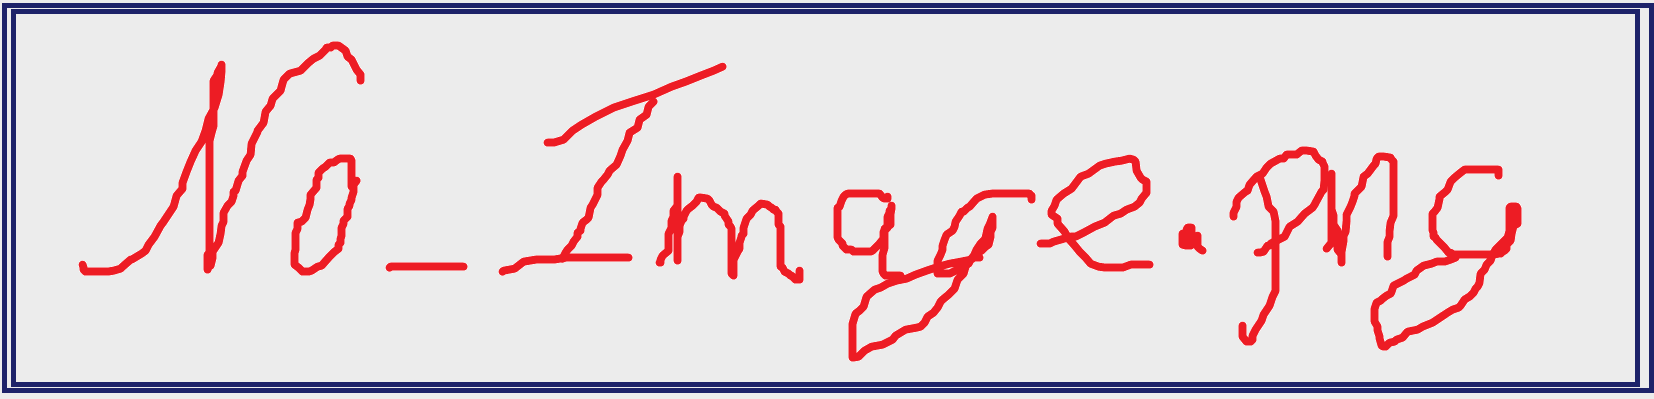
\includegraphics[
		width=\textwidth
	]{figuras/no_image.png}
	\label{fig:TP8-result}
\end{figure}




\end{textocaixa}